% !TEX root = ../../../thesis.tex

% CP1.2H had a mediocre SQUID (sensitivity), in order to improve we moved to SNS junctions as we are more familiar with them.
% Move to a square geometry to improve the coupling.
% Use SiO as a wafer instead of Si to make sure that it does not short through the wafer.

\begin{figure}[ht]
	\begin{subfigure}[t]{0.3\textwidth}
		\centering
		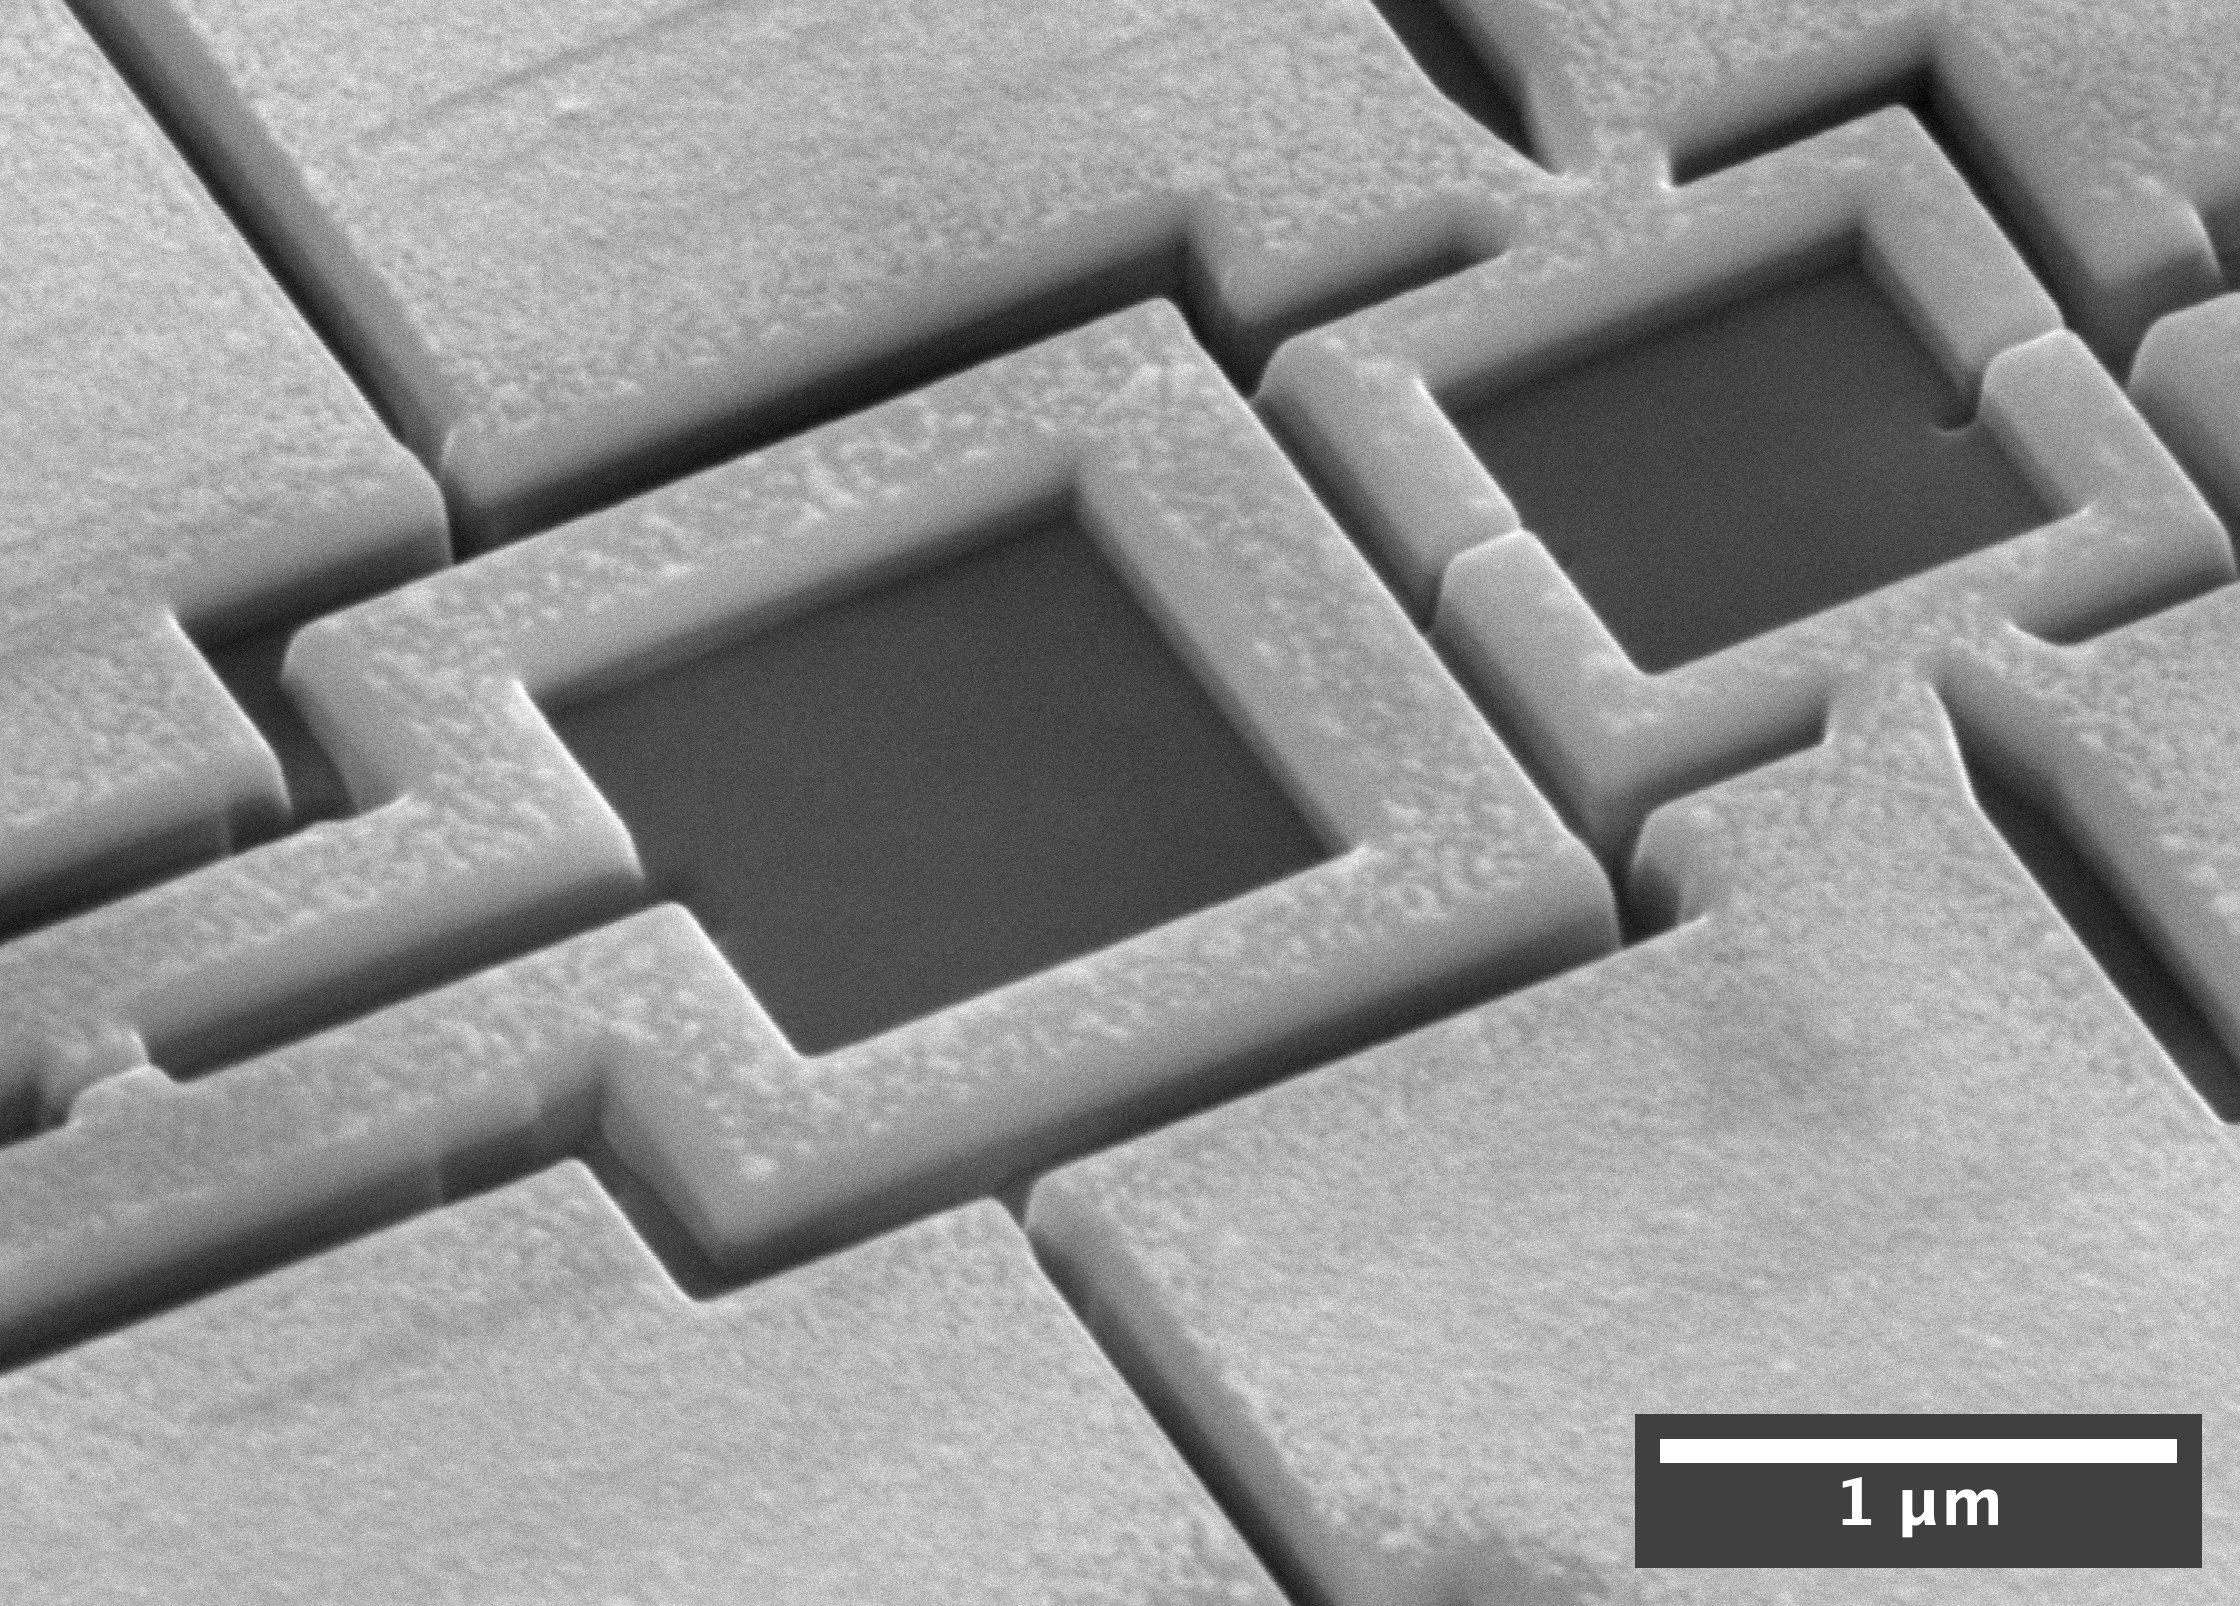
\includegraphics[width=\textwidth]{figures/samples/CP2/CP2.6B_SEM_overview.jpg}
		\subcaption{Overview of the device. The top loop shows the dc-SQUID and the bottom is the junction loop. In-between the arms extending down from the junction loop is the actual Josephson junction under study. The inner and outer diameter of the junction loop are \qty{1.3}{\micro\meter} and \qty{2}{\micro\meter} respectively.}
	\end{subfigure}
	\hfill
	\begin{subfigure}[t]{0.3\textwidth}
		\centering
		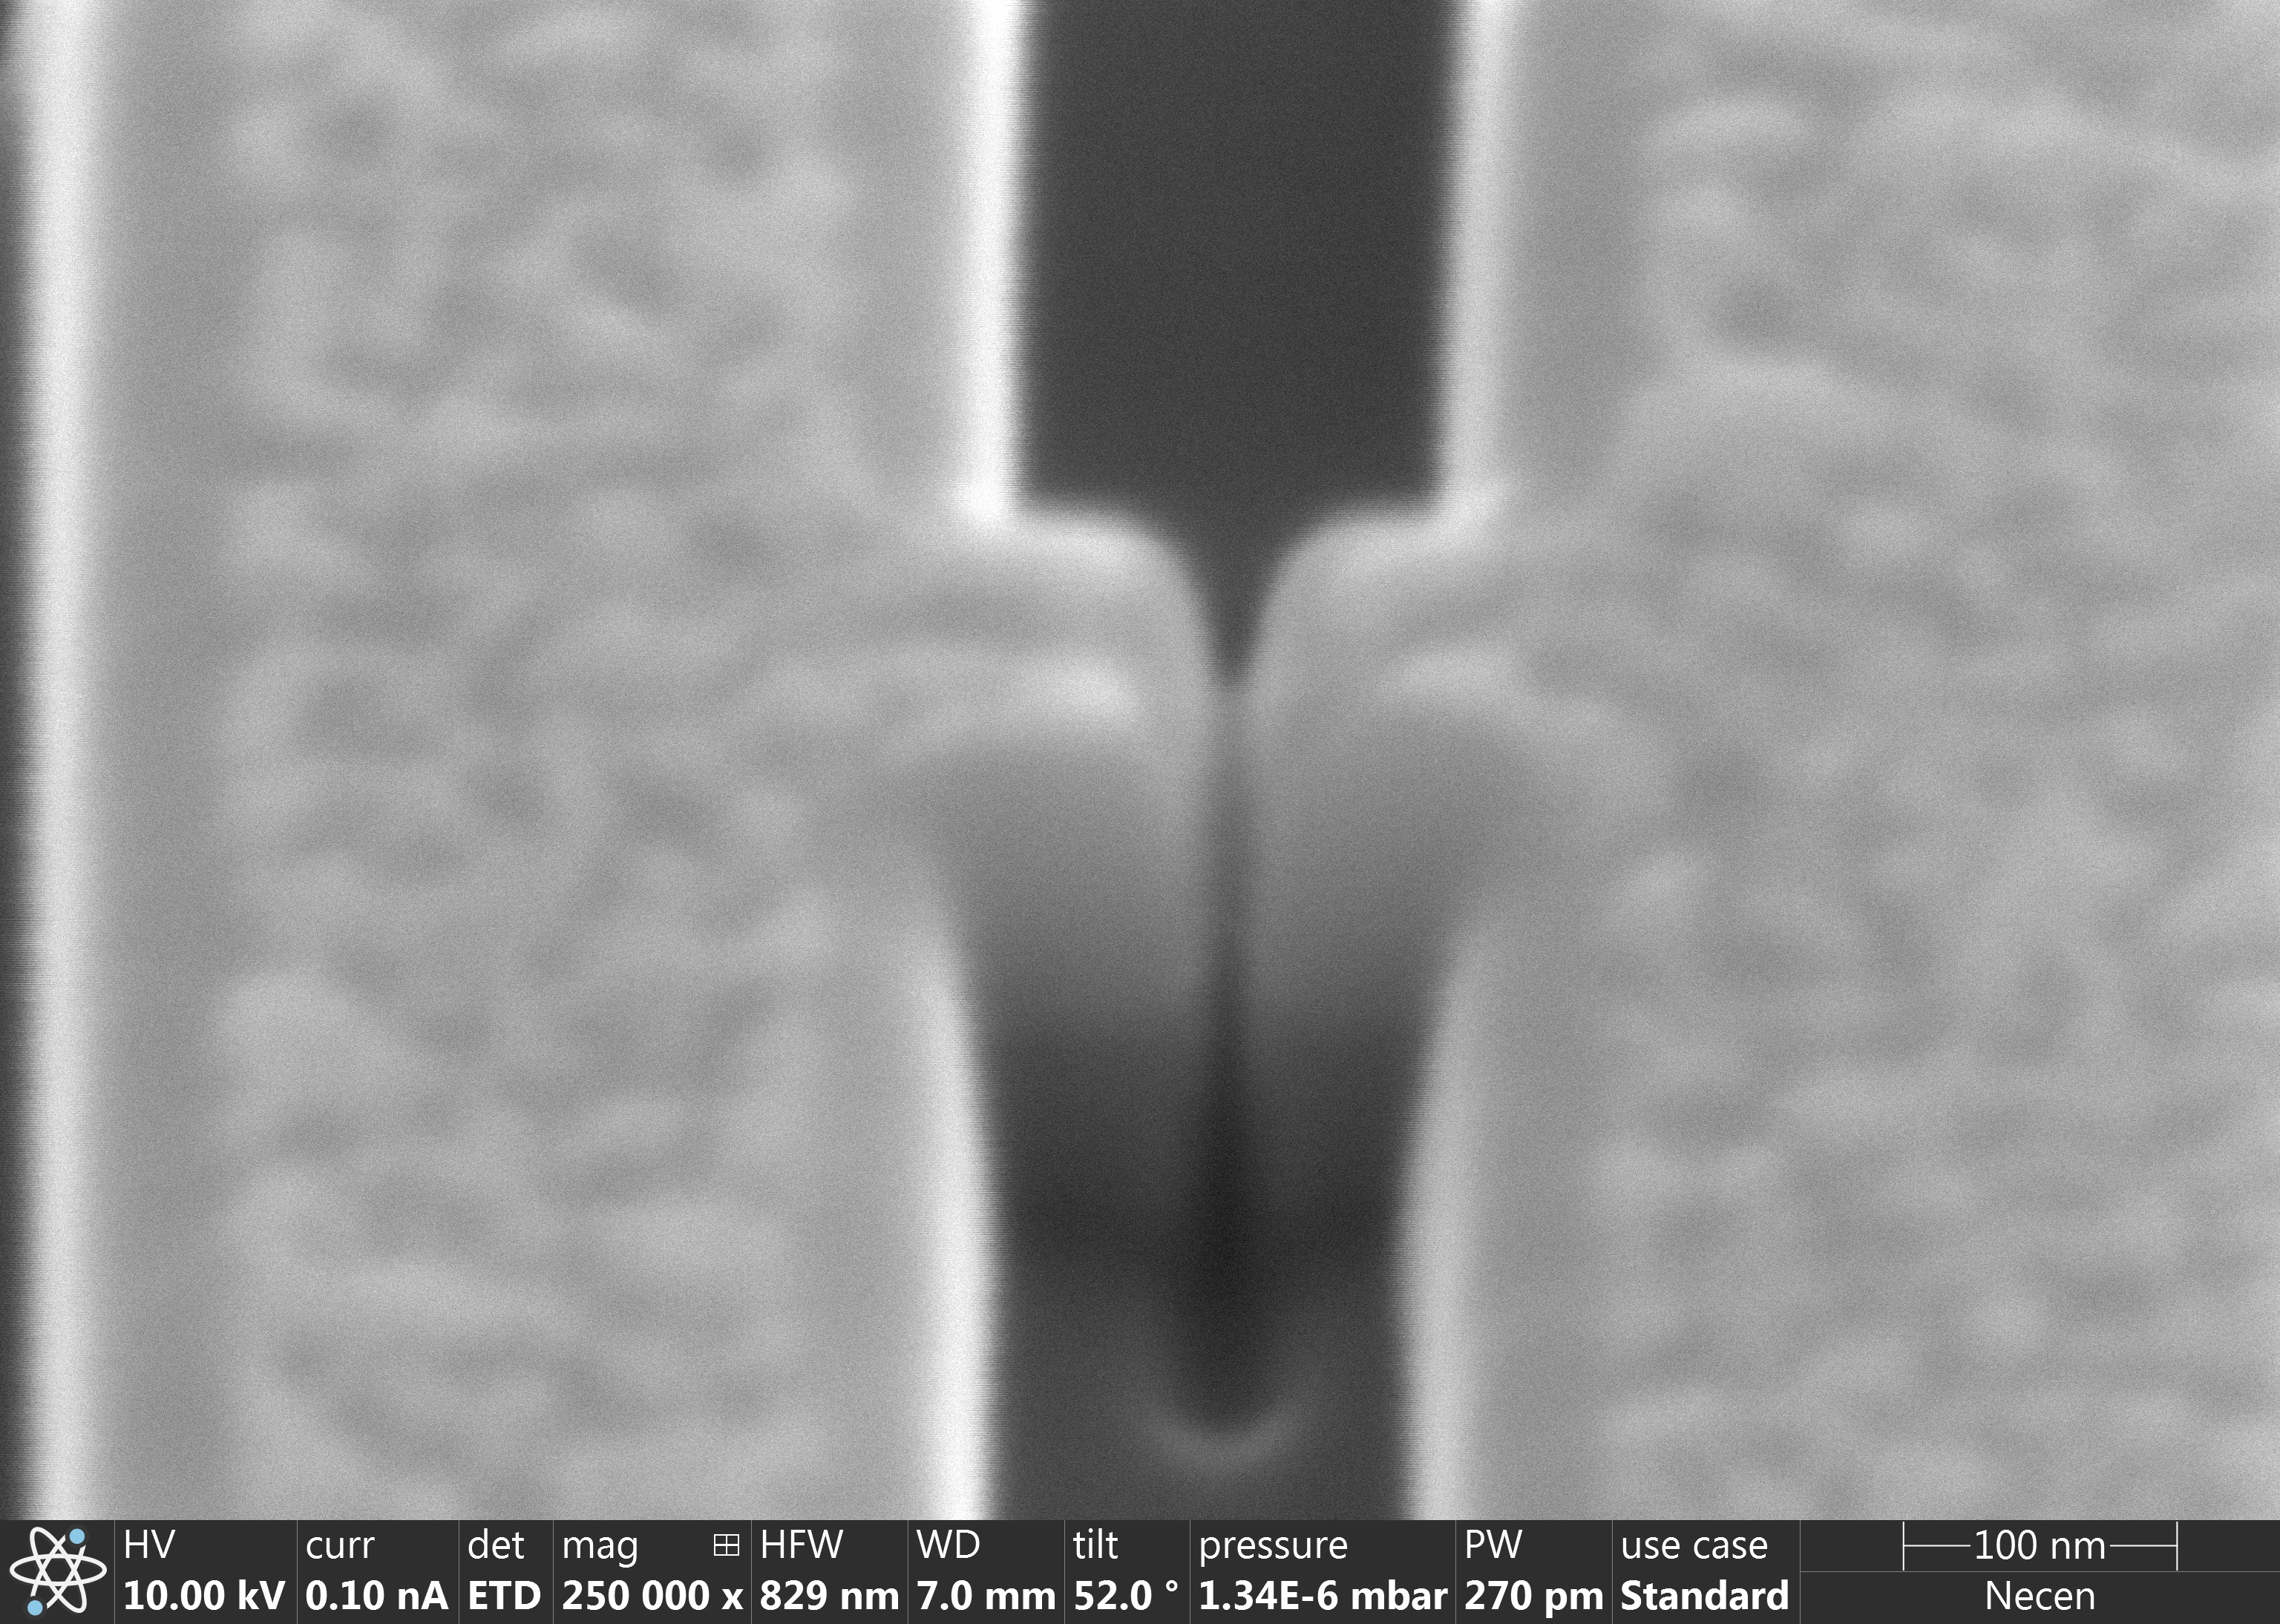
\includegraphics[width=\textwidth]{figures/samples/CP2/CP2.6B_SEM_junction.jpg}
		\subcaption{The Josephson junction under study. The width of the junction is around \qty{12}{\nano\meter}.}
	\end{subfigure}
	\hfill
	\begin{subfigure}[t]{0.3\textwidth}
		\centering
		\includegraphics[width=\textwidth]{figures/samples/CP2/CP2.6B_SEM_SQUID.jpg}
		\subcaption{The dc-SQUID, its inner and outer diameter are \qty{1.0}{\micro\meter} and \qty{1.4}{\micro\meter} respectively. The width of the junctions is \qty{22}{\nano\meter}.}
	\end{subfigure}

	% TODO: fix values.
	\caption{SEM images of sample CP2.6B. The sample consists of a \qty{1}{\nano\meter} of \ce{Cu} sputtered on a \ce{SiO} wafer. On top of the \ce{Cu} is a \qty{1}{\nano\meter} of \ce{Nb}. A final layer of \qty{7}{\nano\meter} of \ce{Au} is used to cap and protect the \ce{Nb}.}
	\label{fig:CP2.6B-SEM-images}
\end{figure}